\chapter{LLM-based Agents}
\label{chap:agents}

In artificial intelligence, an agent is a system that operates autonomously, perceives its environment, persists over time, adapts to change, and creates and pursues goals \cite[Chap.~2]{russellArtificialIntelligenceModern2022}. The associated operational model describes the system as reading its environment through sensors and acting on it through actuators. The agent itself is defined by the mapping between these two interfaces \cite[Chap.~2]{russellArtificialIntelligenceModern2022}. This chapter reviews that classical notion and contrasts it with the LLM-based agent. It then describes how single agents are composed into multi-agent systems and coordinated by the routing pattern this work studies.

\section{The Classical Notion of an Autonomous Agent}
\label{sec:classical-agent}

\subsection{Rationality and the perceive-decide-act loop}
\label{subsec:rationality}

A rational agent selects the action that achieves the best outcome or, when outcomes are uncertain, the best expected outcome \cite[Chap.~2]{russellArtificialIntelligenceModern2022}. Such systems are described by the following elements \cite[Chap.~2]{russellArtificialIntelligenceModern2022}:

\begin{itemize}
	\item The \emph{performance measure}, an external criterion that defines the notion of best by scoring the consequences of the agent's behavior on the environment, specified in terms of states of the world.
	\item The \emph{agent function}, the abstract mapping from percepts to actions, where a percept is the perceptual input available to the agent at a given instant.
	\item The \emph{agent program}, the concrete implementation that produces those actions on a physical or computational machine.
\end{itemize}

Figure~\ref{fig:rational-agent} summarizes these elements and their relations.

\begin{figure}[ht]
	\centering
	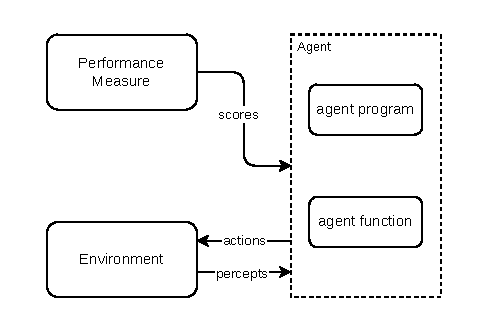
\includegraphics[width=0.6\textwidth]{images/rational_agent.pdf}
	\caption[An autonomous agent]{An autonomous agent}
	\label{fig:rational-agent}
\end{figure}

Independently of its internal design, an agent program implements the same three-step pattern. The system observes the environment, decides what to do, and acts. The action may change the environment; the resulting state is observed, and the cycle repeats. This is the perceive-decide-act loop \cite[Chap.~2]{russellArtificialIntelligenceModern2022}. Rationality is realized in the decide step, where the agent selects the action that, given the available percepts, is expected to maximize the performance measure.

The loop above treats perception as the agent receiving whatever percept the environment provides. Some actions are instead chosen to affect what the agent perceives next rather than to change the state of the environment. This is called information gathering, an action planned for the purpose of reducing the agent's uncertainty about the environment \cite[Chap.~2]{russellArtificialIntelligenceModern2022}. Bajcsy characterizes perception as active, by analogy to biological vision, where the sensing apparatus is continuously adjusted rather than left to record whatever reaches it \cite{bajcsyActivePerception1988}. Under this view, the agent also controls its own data acquisition, through strategies that depend on the goal of the task and on the current state of the interpretation. The choice of what to measure, where to look, and when enough has been observed is formulated as a search that minimizes a loss while seeking the most informative data \cite{bajcsyActivePerception1988}. The control is guided by prior knowledge, in a knowledge-driven regime: the agent's models and expectations direct what it looks for. This has a cost: acquisition can be steered toward what is expected, so unanticipated objects can go undetected \cite{bajcsyActivePerception1988}. The perceive and decide steps are therefore mutually dependent, because the percepts that the decide step acts on are partly the result of earlier choices about what to acquire.

\subsection{Approaches to building agents}
\label{subsec:building-approaches}

Russell and Norvig identify four kinds of agent program that realize the decide step: simple reflex, model-based reflex, goal-based, and utility-based agents \cite[Chap.~2]{russellArtificialIntelligenceModern2022}. Each extends the previous one to remove one of its limitations, and any of the four can in addition be made a learning agent, whose components are acquired from experience instead of being fixed by the designer \cite[Chap.~2]{russellArtificialIntelligenceModern2022}. None of them removes the requirement that the designer specify the task in advance. What changes across the four is the form that the specification takes. Each kind chooses its action from the agent's \emph{current state}, the description of the relevant aspects of the environment at the present instant. A simple reflex agent takes the current state directly from the current percept, but the others reconstruct it from the percept history using a model of the environment \cite[Chap.~2]{russellArtificialIntelligenceModern2022}. Table~\ref{tab:agent-designs} summarizes how each design selects an action, what the designer has to supply, and the limitation that remains.

\begin{itemize}
	\item The \emph{simple reflex agent} realizes the decide step as condition-action rules on the current percept, which works only when the environment is fully observable \cite[Chap.~2]{russellArtificialIntelligenceModern2022}.
	\item The \emph{model-based reflex agent} maintains an internal state to track what the current percept does not reveal, which requires a transition model of how the environment evolves and a sensor model of how its state is reflected in the percepts \cite[Chap.~2]{russellArtificialIntelligenceModern2022}.
	\item The \emph{goal-based agent} adds a description of the desirable situations and selects actions predicted to lead to them, which requires consideration of the future. When a single action does not suffice, this also requires search and planning over a domain model that the designer writes in advance \cite[Chap.~2]{russellArtificialIntelligenceModern2022}. Planning of this kind is computationally costly \cite[Chap.~2]{russellArtificialIntelligenceModern2022}. Hierarchical task network planning reduces the cost by using a plan library of known methods that implement high-level actions, so the planner searches only the sequences allowed by the library instead of the full space of primitive actions \cite[Chap.~11]{russellArtificialIntelligenceModern2022}.
	\item The \emph{utility-based agent} replaces the goal's plain test of whether a state is reached or not with a utility function over states of the world, the internal counterpart of the performance measure, and selects the action that maximizes expected utility \cite[Chap.~2]{russellArtificialIntelligenceModern2022}.
\end{itemize}

Learning is not a separate design for the decide step but a method for improving the components of any of the previous designs \cite[Chap.~2]{russellArtificialIntelligenceModern2022}. A learning agent is decomposed into three components \cite[Chap.~2]{russellArtificialIntelligenceModern2022}. The performance element is the action-selecting program described so far. A learning element modifies it using feedback from a critic, which measures performance against a fixed standard. A problem generator proposes exploratory actions. In its reinforcement-learning instance, the feedback is a reward signal and the agent refines a mapping from percepts to actions through interaction with the environment \cite[Chap.~23]{russellArtificialIntelligenceModern2022}. The cost moves from authoring rules, models, or plans to providing an environment in which to train, a reward function that captures the intended objective, and enough interaction to converge. Dulac-Arnold et al. survey nine challenges that separate laboratory reinforcement learning from production use, including learning from limited samples on the actual system, partial observability and non-stationarity, satisfying safety constraints during training and operation, and specifying a well-posed and aligned reward \cite{dulac-arnoldChallengesRealWorldReinforcement2019}. Each of these typically requires application-specific engineering, and the resulting policy remains tied to the task and to the conditions under which it was trained \cite{dulac-arnoldChallengesRealWorldReinforcement2019}.

\begin{table}[ht]
	\centering
	\small
	\renewcommand{\arraystretch}{1.15}
	\newcolumntype{R}[1]{>{\raggedright\arraybackslash\hsize=#1\hsize}X}
	\begin{tabularx}{\textwidth}{@{}>{\raggedright\arraybackslash}p{2.75cm}R{1.10}R{0.90}R{1.00}@{}}
		\toprule
		Agent type & Action selection & Designer must supply & Principal limitation \\
		\midrule
		Simple reflex & Condition-action rules on the current percept & The rules & Requires a fully observable environment \\
		\addlinespace
		Model-based reflex & Rules over an internal state & Rules, a transition model, a sensor model & No goals and no model of the future \\
		\addlinespace
		Goal-based & Search and planning toward goal states, or refinement from a plan library & A domain model and goals, or a plan library & Planning is costly; competence is bounded by what is authored \\
		\addlinespace
		Utility-based & Maximization of expected utility & A utility function, in addition to a model & The utility function is hard to specify \\
		\addlinespace
		Learning & Any of the above, refined from feedback & A training environment, a reward signal, interaction & The policy is tied to the task and its training conditions \\
		\bottomrule
	\end{tabularx}
	\caption[Comparison of the agent designs]{Comparison of the agent designs.}
	\label{tab:agent-designs}
\end{table}

The decide step is built for a specific task in each of the four designs, whether their components are fixed by the designer or acquired through learning. What the designer must supply is listed in Table~\ref{tab:agent-designs}: the condition-action rules, the transition and sensor models, the domain model and plan library, the utility function, or the training environment and reward signal. Each of these has to be stated in a formal and executable form, over a set of actions fixed in advance, before the agent can act at all.

This requirement is the principal cost of building an agent with these designs. The intended behavior is normally known in informal terms, and the work consists in translating it into a specification that the decide step can execute. This translation demands expertise in the design and in the application domain. It is also incomplete in practice: cases that the specification does not cover produce no useful behavior, and the effort grows with the range of cases that the agent has to handle. The reinforcement-learning case illustrates the same cost in a different form, since the reward signal has to express the intended objective and the training conditions have to reproduce the operating conditions. Each of these requires application-specific engineering \cite{dulac-arnoldChallengesRealWorldReinforcement2019}. Building an agent under these designs is therefore limited less by the loop of Section~\ref{subsec:rationality} than by the difficulty of producing the specification that the decide step needs.

\section{The Language Model as Agent Core}
\label{sec:llm-decision-component}

The approaches described in Section~\ref{sec:classical-agent} share the property summarized in Table~\ref{tab:agent-designs}: the decide step is constructed for each task from rules, models, plans, utility functions, or trained policies, authored or trained by the designer over a closed set of actions and against an explicit specification. In contrast to these approaches, a more recent line of work realizes the decide step with a pretrained large language model, of the kind described in Chapter~\ref{chap:llm}, which serves as the agent's core computation unit \cite{zhaoSurveyLargeLanguage2026}. The resulting systems are referred to here as LLM-based agents. They do not build the decide step for any one task: the task is supplied to the model as input, in natural language, rather than encoded into the decide step in advance. This changes what the designer has to produce, since the desired behavior is stated in the terms in which it is normally known, instead of being translated into rules, models, plans, utility functions, or reward signals. It does not remove the design work, and it raises the separate problem of checking that the desired behavior is the behavior obtained, which Chapter~\ref{chap:evaluating-agents} addresses. Models of this kind have emerged as the decision component of agents \cite{zhaoSurveyLargeLanguage2026}, and the volume of literature on them has grown in recent years \cite{wangSurveyLargeLanguage2024}.

\subsection{The language model as the decide step}
\label{subsec:new-decide-step}

The instruction-tuned model of Section~\ref{sec:scale-emergence} is a stochastic policy that takes a prompt as input, emits a token sequence as output, and generalizes across tasks without being retrained for each one \cite{ouyangTrainingLanguageModels2022}. Because it is a foundation model adaptable across tasks \cite{bommasaniOpportunitiesRisksFoundation2022}, what varies from one agent to another is the prompt that frames the goal, the external operations the agent is allowed to invoke, and the data retrieved into its context, rather than the model itself. The same model can be used inside a coding agent, a customer-support agent, or a research assistant. Constructing a new agent remains an engineering task, but it modifies the inputs supplied to the model rather than the decide step it implements.

The definition of agents given by Anthropic is representative, as it groups workflows and agents together as agentic systems while drawing an architectural distinction between them \cite{BuildingEffectiveAI}:

\begin{quotebox}
``Agent'' can be defined in several ways. Some customers define agents as fully autonomous systems that operate independently over extended periods, using various tools to accomplish complex tasks. Others use the term to describe more prescriptive implementations that follow predefined workflows. At Anthropic, we categorize all these variations as \textbf{agentic systems}, but draw an important architectural distinction between \textbf{workflows} and \textbf{agents}:
\begin{itemize}
	\item Workflows are systems where LLMs and tools are orchestrated through predefined code paths.
	\item Agents, on the other hand, are systems where LLMs dynamically direct their own processes and tool usage, maintaining control over how they accomplish tasks.
\end{itemize}
\end{quotebox}

This distinction is consistent with the one adopted in Section~\ref{sec:classical-agent}, where an agent is distinguished by controlling how it pursues its goal.

\subsection{Tools and perception}
\label{subsec:llm-tools-perception}

Realizing the decide step with a large language model also governs the perceive step. Within the context window, all content is treated uniformly as input. A user instruction, a retrieved document, the output of a previous step, and the result returned by a tool all enter the context as text and affect what the model produces next. Percepts reach the model along two routes:

\begin{itemize}
	\item \textbf{Supplied percepts.} These reach the model without the model taking part in their selection: the user request, an event reported by the environment, or a document placed in the context before the model runs.
	\item \textbf{Obtained percepts.} These are retrieved by the model itself. Through the function-calling interface of Section~\ref{sec:structured-output}, the model can emit a structured call to a tool instead of a final action, and the result of that call returns to the context as the next percept.
\end{itemize}

The exchange of a tool call and its returned result recurs across steps, forming the loop described in Section~\ref{subsec:tool-use-react}. In this loop, not every tool call serves the same purpose. Tool calls may be aimed to:

\begin{itemize}
	\item \textbf{Take actions.} A call issued to change the state of the environment.
	\item \textbf{Gather information.} A call issued only to obtain information the model lacks, without changing the environment, such as reading a file or querying a document store. This is the information gathering of Section~\ref{subsec:rationality}: an action planned to reduce the model's uncertainty about the environment rather than to change it.
\end{itemize}

It is this second kind of call that realizes the active perception of Section~\ref{subsec:rationality}. What is available at a given step is therefore in part the result of the model's own earlier choices. Because of that, the perceive, decide, and act steps are not three phases executed once per iteration, but three processes that overlap in time. Issuing a call is a decision. The call is an action when it changes the environment, and an act of perception when it only retrieves information. The result it returns reopens perception, which feeds the next decision in turn. The dependence on prior knowledge described in Section~\ref{subsec:rationality} applies here as well, where expectations assist interpretation but carry the danger of finding what is expected and not detecting what is not \cite{bajcsyActivePerception1988}.

\subsection{Limitations}
\label{subsec:llm-agent-fit}

LLM-based agents replace the rules, models, plans, utility functions, or reward signals of the classical designs with natural-language instructions, which are easier to define and maintain, but do not carry the same precision or expressiveness: a rule or a reward signal has fixed, unambiguous semantics, while a natural-language instruction can be interpreted differently by the model, or interpreted inconsistently across invocations.

The properties defined in Section~\ref{sec:properties} are also inherited by LLM-based agents, since every step of the perceive-decide-act loop is the output of a model call. The action taken at a step is non-deterministic. The policy the agent is meant to apply, stated as prompt instructions, may not be followed, or only partially followed. As the content supplied to the agent grows, performance may degrade, depending on its length and on the position of the relevant information in it. An agent can also hallucinate information and state it with confidence.

Operating in a loop compounds these properties. Each step's output feeds into the context of later steps, so a non-deterministic choice, an unfollowed instruction, or a hallucination at one step propagates to the steps that follow it \cite{wangSurveyLargeLanguage2024}.

The classical designs provide two guarantees by construction: a fixed action set and an explicit specification of when each action applies. Neither guarantee is available here. The specification is easier to write, and conformance to it is no longer established by construction. Whether the behavior obtained matches the desired behavior has to be determined by observing the system. This is the subject of Chapter~\ref{chap:evaluating-agents}.

\section{Anatomy of an LLM-based Agent}
\label{sec:agent-anatomy}

An LLM-based agent is built around a small set of recurring components: tool use, memory, and planning. Tool use is the defining component, since it extends the language model from a system that emits text to one that can act on its environment. Together, these components produce the trajectory, the ordered sequence of reasoning steps, tool calls, and intermediate outputs that the agent goes through before it returns a final response. The trajectory is the unit on which later evaluation operates.

\subsection{The ReAct loop}
\label{subsec:tool-use-react}

ReAct, short for reasoning and acting, is a method that connects language models to the classical notion of an autonomous agent, later turned into a first-class abstraction by the function-calling interface of Section~\ref{sec:structured-output} \cite{yaoReActSynergizingReasoning2022, FunctionCallingOther2024}. The method described in the paper consists of a prompting technique that prompts the model to generate reasoning traces and task-specific actions in an interleaved manner. On the two interactive decision-making benchmarks ALFWorld and WebShop, it improved the absolute success rate over imitation and reinforcement learning baselines by 34\% and 10\% respectively, while using only one or two in-context examples \cite{yaoReActSynergizingReasoning2022}. The action space is augmented to
\begin{equation}
    \hat{A} = A \cup L,
\end{equation}
where
\begin{itemize}
    \item $A$ is the set of domain actions;
    \item $L$ is the space of language \cite{yaoReActSynergizingReasoning2022}.
\end{itemize}
$L$ is the language the model produces as output. An action drawn from $L$, called a thought, does not affect the environment and produces no observation: it lets the model induce, track, and update plans, handle exceptions, and compose information by reasoning over the current context, updating that context for the steps that follow \cite{yaoReActSynergizingReasoning2022}. An action drawn from $A$ interfaces with an external source, such as a weather API, and returns information into the context. In the original formulation, a frozen language model is prompted with few-shot examples to emit both thoughts and actions, producing a trajectory of interleaved thought, action, and observation steps, with no runtime component beyond the prompt \cite{yaoReActSynergizingReasoning2022}. Figure~\ref{fig:react-example} shows such a trajectory for a query about the weather in the user's city, where the model first retrieves the city and then queries the weather for it.

\begin{figure}[ht]
	\centering
	\vspace{4mm}
	\begin{tikzpicture}[
		node distance=5mm,
		every node/.style={font=\small},
		thought/.style={draw, dashed, rounded corners, align=left, text width=0.82\textwidth, inner sep=5pt},
		action/.style={draw, rounded corners, align=left, text width=0.82\textwidth, inner sep=5pt},
		obs/.style={align=left, text width=0.82\textwidth, inner sep=5pt, font=\small\itshape},
		query/.style={draw, thick, rounded corners, align=left, text width=0.82\textwidth, inner sep=5pt, font=\small\bfseries},
		arr/.style={-{Latex[length=2mm]}}
		]
		\node[query] (q) {Query: What is the weather in my city?};
		\node[thought, below=of q] (t1) {[L] Thought 1: The query asks for the weather in the user's city, but the city is not in the context. I should look it up first.};
		\node[action, below=of t1] (a1) {[A] Action 1: \texttt{get\_location[]}};
		\node[obs, below=of a1] (o1) {Observation 1: city is London};
		\node[thought, below=of o1] (t2) {[L] Thought 2: The city is London. Now I can check the weather for it.};
		\node[action, below=of t2] (a2) {[A] Action 2: \texttt{get\_weather[London]}};
		\node[obs, below=of a2] (o2) {Observation 2: 22\textdegree C, partly cloudy};
		\node[thought, below=of o2] (t3) {[L] Thought 3: The weather in London is now known, so the query can be answered.};
		\node[action, below=of t3] (a3) {[A] Action 3: \texttt{finish[22\textdegree C, partly cloudy in London]}};
		\foreach \x/\y in {q/t1, t1/a1, a1/o1, o1/t2, t2/a2, a2/o2, o2/t3, t3/a3}
			\draw[arr] (\x) -- (\y);
	\end{tikzpicture}
	\caption[An example ReAct trajectory for a weather query]{An example ReAct trajectory for a weather query.}
	\label{fig:react-example}
\end{figure}

In the function-calling interface, each action of Figure~\ref{fig:react-example} becomes a declared function call, such as \texttt{get\_weather(city="London")}, and each observation becomes the value the runtime returns. This interface is architecturally similar to the thought, action, and observation cycle of ReAct, but it separates the concerns of the cycle. The model first declares intent by selecting a function and its arguments, then the runtime executes the call, and the result is injected back into the context as the next input. ReAct couples the generation of the action and its execution within the prompt and the surrounding environment, but function calling assigns execution to the runtime and leaves the model responsible only for declaring the call. Figure~\ref{fig:react-loop} shows the loop as implemented with function calling.

\begin{figure}[ht]
	\centering
	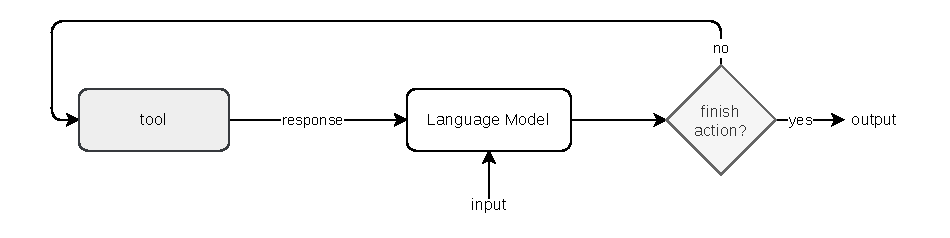
\includegraphics[width=0.92\textwidth]{images/react_loop.pdf}
	\caption[The ReAct loop with tool calling]{The ReAct loop with tool calling}
	\label{fig:react-loop}
\end{figure}

This loop matches the perceive-decide-act cycle of the classical agent of Section~\ref{sec:classical-agent}. The model carries out the decide step; the environment executing a call realizes the act step; the returned response supplies the perceive step. Table~\ref{tab:classical-llm} extends the same correspondence to every component, mapping the elements of the formulation of Russell and Norvig onto their counterparts in an LLM-based agent.
\begin{table}[ht]
	\centering
	\small
	\begin{tabularx}{\textwidth}{@{}XX@{}}
		\toprule
		Classical agent & LLM-based agent \\
		\midrule
		Percept & Content entering the context, including tool results \\
    Actions & Tool calls \\
		Agent function & A forward pass of the language model \\
		Internal state & Context window \\
		Performance measure & External evaluation criterion, applied after the run \\
		\bottomrule
	\end{tabularx}
	\caption[Correspondence between classical agent and LLM-based agents]{Correspondence between classical agent and LLM-based agents.}
	\label{tab:classical-llm}
\end{table}

The performance measure of Section~\ref{subsec:rationality} drives action selection during the run, since the decide step selects the action expected to maximize it \cite[Chap.~2]{russellArtificialIntelligenceModern2022}. An LLM-based agent has no such measure active during the run. It is not built for one task and its objective is defined in the prompt as natural language; therefore, no criterion over states is available to it while it runs. The criterion is applied only after the run, by an evaluation setup that decides both what to evaluate and how to evaluate it \cite{mohammadiEvaluationBenchmarkingLLM2025}. Chapter~\ref{chap:evaluating-agents} describes how such a criterion is defined.

\subsection{Building blocks}
\label{subsec:building-blocks}

So far, the minimal agent has been defined by a language model, a set of tools, and the loop that connects them. On a higher level of abstraction, the loop and the tool definitions allow the agent to be described as a set of components organized around the language model. Zhao et al. and Wang et al. converge on the same three: memory, planning, and an execution component that carries out the plan, called action by Wang et al. \cite{zhaoSurveyLargeLanguage2026, wangSurveyLargeLanguage2024}. Zhao et al. describe the language model as the core computation unit, equipped with these three components and integrated under its control during interactions with the environment \cite{zhaoSurveyLargeLanguage2026}. Wang et al. add a fourth module, profiling, which identifies the role of the agent and influences the memory and planning modules; those two modules, together with profiling, in turn influence the action module \cite{wangSurveyLargeLanguage2024}. The three shared modules are described below. The ReAct loop of Section~\ref{subsec:tool-use-react} sequences their use.

\paragraph{Planning.} The planning component decomposes a complex task into simpler subtasks that are solved individually \cite{wangSurveyLargeLanguage2024}. Wang et al. separated existing designs according to whether the agent receives feedback during the planning process \cite{wangSurveyLargeLanguage2024}:
\begin{itemize}
    \item \emph{Planning without feedback}, where the agent does not receive feedback that can influence its future behavior after taking actions. This covers single-path reasoning, in which the task is decomposed into intermediate steps connected in a pipeline, each leading to a single subsequent step. It also covers multi-path reasoning, in which the steps are organized into a tree and each step may have several subsequent steps, and the delegation of plan generation to a well-developed external planner \cite{wangSurveyLargeLanguage2024}.
    \item \emph{Planning with feedback}, where the agent revises its plans after taking actions on the basis of signals obtained from the environment, from humans, or from a model. This is better suited to complex tasks that need long-horizon planning, where planning without feedback is less effective \cite{wangSurveyLargeLanguage2024}.
\end{itemize}

\paragraph{Memory.} The memory component stores information perceived from the environment and uses the recorded memories to facilitate future actions \cite{wangSurveyLargeLanguage2024}. Wang et al. analyzed it along three perspectives \cite{wangSurveyLargeLanguage2024}:
\begin{itemize}
    \item \emph{Structures}, which distinguish short-term from long-term memory. Short-term memory consists of the information within the context window constrained by the transformer architecture, while long-term memory resembles an external store that the agent can query and retrieve from as needed.
    \item \emph{Formats}, the medium in which the content is stored, including raw natural language, embedding vectors, databases, and structured lists \cite{wangSurveyLargeLanguage2024}.
    \item \emph{Operations}, through which the component interacts with the environment: \textbf{reading}, which extracts relevant information from memory to inform the next action; \textbf{writing}, which stores new information while handling duplication and storage limits; and \textbf{reflection}, which summarizes past records into higher-level insights \cite{wangSurveyLargeLanguage2024}.
\end{itemize}

\paragraph{Action.} The action component translates the agent's decisions into specific outcomes and is located at the most downstream position, where it directly interacts with the environment \cite{wangSurveyLargeLanguage2024}. Two of the perspectives used by Wang et al. bear on the runtime structure \cite{wangSurveyLargeLanguage2024}:
\begin{itemize}
    \item The \emph{action space}, the set of actions available to the agent, divided into external tools and what the model already knows from training. External tools include APIs, databases and knowledge bases, and other models, each of which expands the action space beyond the limitations of the language model on its own \cite{wangSurveyLargeLanguage2024}.
    \item The \emph{action impact}, the consequence of an action, which may change the environment, alter the agent's own internal state such as its memory or plans, or trigger further actions \cite{wangSurveyLargeLanguage2024}.
\end{itemize}

Systems with more than one specialized function add a routing mechanism. It governs the flow of control to different specialized functions, tools, or sub-processes. Through it, the agent evaluates specific criteria and selects from a set of possible subsequent actions instead of following a fixed execution path \cite[Chap.~2]{gulliAgenticDesignPatterns2025}.

Figure~\ref{fig:agent-blocks} shows the complete agent: the language model receives an input and produces a response, drawing on planning and memory and issuing tool calls that act on the environment.

\begin{figure}[ht]
	\centering
	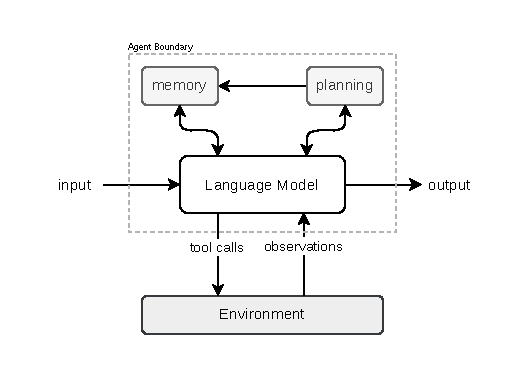
\includegraphics[width=0.75\textwidth]{images/agent_blocks.pdf}
	\caption[The complete LLM-based agent with its building blocks]{The complete LLM-based agent with its building blocks}
	\label{fig:agent-blocks}
\end{figure}

\subsection{Memory and retrieval}
\label{subsec:memory-reml}

The long-term part of the memory component rests on information retrieval. Wang et al. distinguished a unified structure from a hybrid structure \cite{wangSurveyLargeLanguage2024}. A unified structure holds only the short-term memory of Section~\ref{subsec:building-blocks}, directly in the context window. A hybrid structure adds long-term memory: it retrieves relevant records from an external store and inserts them into the prompt, governed by the reading operation and its relevance scoring \cite{wangSurveyLargeLanguage2024}. Retrieval-augmented generation implements this scheme by retrieving relevant information from an external knowledge base, which reduces the generation of factually incorrect content and allows continuous knowledge updates and the integration of domain-specific information \cite{gaoRetrievalAugmentedGenerationLarge2024}. Retrieval introduces failure modes of its own: low precision leads to the selection of misaligned or irrelevant content, and low recall leads to missing crucial information \cite{gaoRetrievalAugmentedGenerationLarge2024}. The model may still produce content not supported by the retrieved context, and it may echo retrieved content without synthesizing it \cite{gaoRetrievalAugmentedGenerationLarge2024}. What enters the context through memory affects every subsequent step, so an error in retrieval propagates through the rest of the loop.

\subsection{Role and configuration}
\label{subsec:agent-identity}

Section~\ref{subsec:new-decide-step} shows that constructing a new agent means changing the prompt, the tools, and the retrieved context, not the model itself. Multiple agents can therefore share the same underlying model and still be told apart, which raises the question of what distinguishes one agent from another, and of whether an agent whose prompt or toolset has changed still counts as the same agent.

The profiling module of Section~\ref{subsec:building-blocks} identifies an agent by its \emph{role}, such as planner, speaker, coordinator, or specialist, written into the prompt to shape the model's behavior \cite{wangSurveyLargeLanguage2024}. Wang et al. use this to populate a system with several distinct agents, for example assigning software-development roles to a collaborating team or generating a population of agents for social simulation \cite{wangSurveyLargeLanguage2024}. In their examples, the role is what tells two agents in the same system apart.

The role and the configuration answer this at two different levels of abstraction, and the two coexist:

\begin{itemize}
	\item At a higher level of abstraction, an agent is defined by the role it occupies, and stays the same agent across a change to its configuration, as long as it keeps the same role.
	\item At a lower level of abstraction, an agent is defined by the prompt, the underlying model, and the toolset made available to it.
\end{itemize}

\section{Multi-Agent Systems}
\label{sec:multi-agent}

A single LLM-based agent, built as in Section~\ref{sec:agent-anatomy}, has limits that grow with the difficulty of the task. Its short-term memory is the information inside the context window, and the transformer architecture bounds it \cite{wangSurveyLargeLanguage2024}. Multi-agent orchestration answers this with a paradigm in which specialized agents assume distinct roles, exchange information through structured protocols, and coordinate their actions to solve problems beyond the reach of any single agent \cite{zhuLLMBasedMultiAgentOrchestration2026a}. Compared with a system that uses a single LLM-based agent, this paradigm specializes LLMs into distinct agents, each with different capabilities, that interact with each other \cite{guoLargeLanguageModel2024}. Section~\ref{sec:coordinator} examines the coordinator-based routing pattern this work studies, in which a coordinator assigns each query to a specialized agent.

Zhu et al. defined the \emph{coordination topology} of a multi-agent system as the directed graph whose vertices are the agents and whose edges are the message-passing or delegation pathways declared at design time \cite{zhuLLMBasedMultiAgentOrchestration2026a}. This graph expresses which agent may direct another, and along which paths messages flow between agents. Their taxonomy has three topologies: centralized, where the graph is a star with a designated supervisor; decentralized, where it is a peer graph with no designated supervisor; and hierarchical, where it is a tree \cite{zhuLLMBasedMultiAgentOrchestration2026a}.

A second axis of the same taxonomy is runtime adaptivity. Here, the active edges are the subset of the topology's edges that carry a message at a given step, distinct from the full edge set declared at design time. A system is static when its vertices, its active edges, and its routing policy are fixed at design time and do not change for the duration of a task, and dynamic-adaptive when that configuration changes at run time, for instance when only the active edge subset changes while the vertices and the permitted edges stay fixed \cite{zhuLLMBasedMultiAgentOrchestration2026a}. The axis is orthogonal to the topology, so any of the three topologies can be static or dynamic-adaptive \cite{zhuLLMBasedMultiAgentOrchestration2026a}.

\subsection{Centralized}
\label{subsec:topology-centralized}

A single supervisor agent owns the workflow: it decomposes the incoming task, assigns subtasks to worker agents, collects their outputs, and decides what happens next \cite{zhuLLMBasedMultiAgentOrchestration2026a}. Every message passes through the supervisor, which therefore keeps a global view of the progress of the task, and the supervisor is typically a language model that reads the current state to select the next worker \cite{zhuLLMBasedMultiAgentOrchestration2026a}. Guo et al. described the same shape as centralized communication, where a central agent coordinates the communication of the system and the other agents interact through this central node \cite{guoLargeLanguageModel2024}. The supervisor is also a single point of failure and a throughput bottleneck, and its context window fills as the number of agents and the length of the conversation grow, which makes the topology suitable for a modest number of agents, roughly three to seven \cite{zhuLLMBasedMultiAgentOrchestration2026a}.

\begin{figure}[ht]
	\centering
	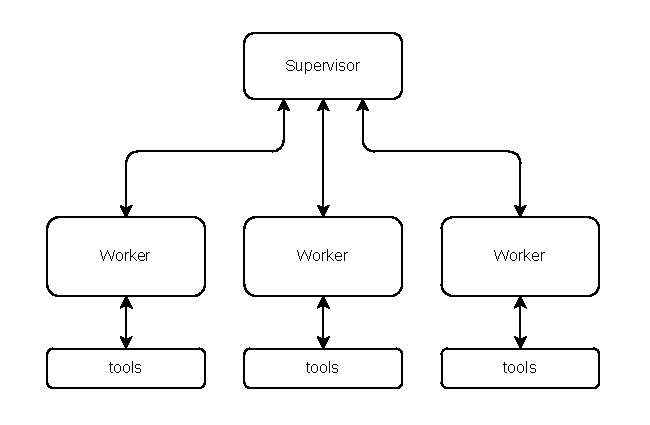
\includegraphics[width=0.72\textwidth]{images/topology_centralized.pdf}
	\caption[Centralized topology]{Centralized topology}
	\label{fig:topology-centralized}
\end{figure}

\subsection{Decentralized}
\label{subsec:topology-decentralized}

No central coordinator exists. The agents communicate directly, and each one decides on its own when to act, whom to consult, and how to contribute. Task allocation emerges from negotiation and self-selection, with each agent holding local state and taking its own routing decisions \cite{zhuLLMBasedMultiAgentOrchestration2026a}. Guo et al. described the same shape as decentralized communication, which operates on a peer-to-peer network where agents communicate directly with each other \cite{guoLargeLanguageModel2024}. They called the corresponding interaction style the debate paradigm, where agents present and defend their own viewpoints or solutions and criticize those of the others to reach a consensus or a more refined solution \cite{guoLargeLanguageModel2024}. The topology removes the single point of failure and lets solutions emerge from unconstrained interaction, but coherent global behavior is hard to guarantee and distributed execution traces make later debugging laborious \cite{zhuLLMBasedMultiAgentOrchestration2026a}. The absence of a single control point also places this topology outside the scope of the routing pattern this work studies, since there is no vertex at which a coordination decision of the kind defined in Section~\ref{sec:coordinator} could be located.

\begin{figure}[ht]
	\centering
	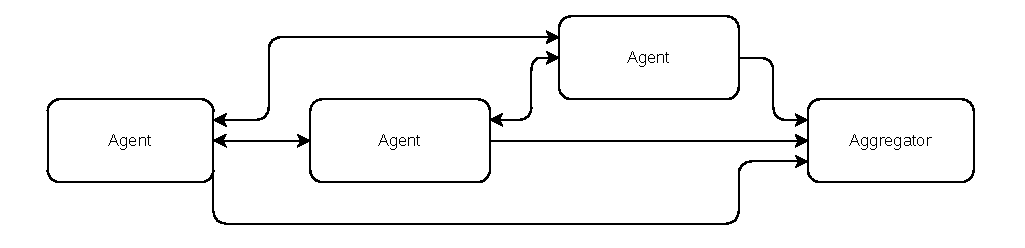
\includegraphics[width=0.88\textwidth]{images/topology_decentralized.pdf}
	\caption[Decentralized topology]{Decentralized topology}
	\label{fig:topology-decentralized}
\end{figure}

\subsection{Hierarchical}
\label{subsec:topology-hierarchical}

The agents are organized in a tree. Manager agents assign subtasks to the level below, and results return to the level above; this is assignment as defined in Section~\ref{sec:coordinator}, since a manager continues the work once its subordinate reports back. Each manager covers one domain or subtask scope and may decompose its assignment further, so top-level managers assign subtasks to mid-level managers and these assign subtasks to leaf-level workers \cite{zhuLLMBasedMultiAgentOrchestration2026a}. An agent that is a worker for its parent is therefore a manager for its own children, and the decision taken once by the supervisor of Figure~\ref{fig:topology-centralized} is repeated at every internal node. Communication scales linearly within the tree rather than quadratically across the full set of agents. This suits large decomposable tasks and systems that must grow beyond ten to fifteen agents, at the cost of the latency of multi-level message passing \cite{zhuLLMBasedMultiAgentOrchestration2026a}. Intermediate managers also become bottlenecks when the tree is not balanced \cite{zhuLLMBasedMultiAgentOrchestration2026a}. Guo et al. described the same shape as layered communication, where agents at each level have distinct roles and interact within their layer or with adjacent layers \cite{guoLargeLanguageModel2024}. Magentic-One extends the pattern with a lead orchestrator that plans, tracks progress, and replans to recover from errors, directing specialized agents for web browsing, file navigation, and code execution \cite{zhuLLMBasedMultiAgentOrchestration2026a}.

\begin{figure}[ht]
	\centering
	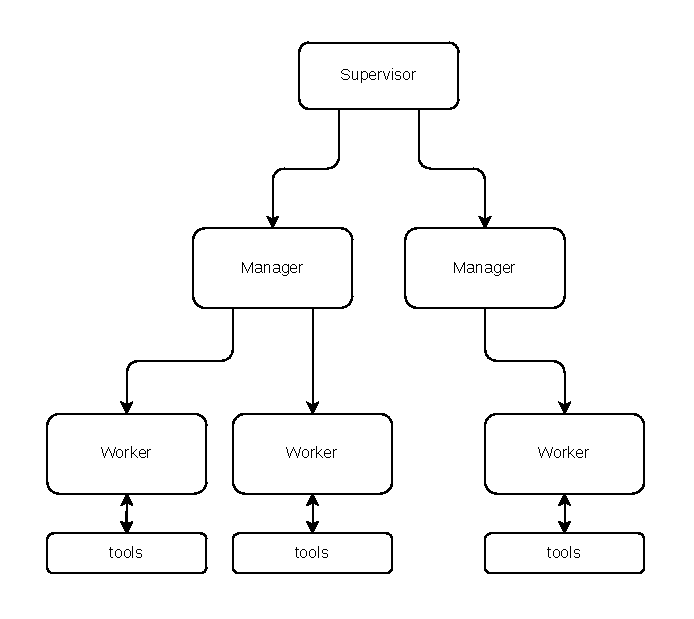
\includegraphics[width=0.7\textwidth]{images/topology_hierarchical.pdf}
	\caption[Hierarchical topology]{Hierarchical topology}
	\label{fig:topology-hierarchical}
\end{figure}



\subsection{Orchestration frameworks}
\label{subsec:topology-frameworks}

These topologies are not merely descriptive categories: they are the constructs that current frameworks expose. Zhu et al. observed that, without a dedicated orchestration layer, agents show three canonical failure modes:
\begin{itemize}
	\item task duplication, where several agents solve the same subtask independently;
	\item contradictory outputs, where agents produce inconsistent artifacts from shared premises;
	\item convergence failure, where the system cycles indefinitely without reaching a terminal state \cite{zhuLLMBasedMultiAgentOrchestration2026a}.
\end{itemize}
The frequency and the severity of these failures increase with the number of agents and the complexity of the task, which is why Zhu et al. treated orchestration as a first-class engineering concern and not as an implementation afterthought \cite{zhuLLMBasedMultiAgentOrchestration2026a}. Every major framework exposes configuration options for it, in the form of speaker-selection policies, delegation flags, conditional edges, and manager swaps. Most frameworks are therefore not restricted to a single cell of the taxonomy and instead cover a small contiguous region of it, with one primary cell obtained from the documented defaults and adjacent cells reachable through configuration \cite{zhuLLMBasedMultiAgentOrchestration2026a}.

\section{The Coordinator Pattern}
\label{sec:coordinator}

Most of the topologies of Section~\ref{sec:multi-agent} require a decision on which agent receives a given unit of work, and the literature names the component that takes it differently depending on the topology: supervisor in a centralized topology, manager at any level of a hierarchical topology \cite{zhuLLMBasedMultiAgentOrchestration2026a}. Both perform the same function, so this work fixes one term for it regardless of topology. Table~\ref{tab:coordinator-terms} defines the terminology used from this point on, \emph{coordinator} for the component that takes the decision, \emph{routing} for the decision itself, and \emph{sub-agent} for each specialized agent it can select, together with the synonyms each term replaces. Those synonyms belong to the topology-specific vocabulary of Section~\ref{sec:multi-agent} and to the source it is drawn from \cite{zhuLLMBasedMultiAgentOrchestration2026a}; they are not used elsewhere in this work.

\begin{table}[ht]
	\centering
	\small
	\renewcommand{\arraystretch}{1.4}
	\begin{tabularx}{\textwidth}{@{} l >{\raggedright\arraybackslash}X >{\raggedright\arraybackslash}p{3.1cm} @{}}
		\toprule
		Term & Role & Synonyms \\
		\midrule
		Coordinator & Reads the request, classifies it against the declared sub-agents, and selects exactly one. & Supervisor (centralized topology), manager (hierarchical topology) \\
		Sub-agent & Specialized agent that a coordinator can select; acts under its own instructions and tools once selected. & Worker \\
		Routing & The decision the coordinator takes. & --- \\
		Handoff & The act of passing the request to the selected sub-agent. & --- \\
		Assignment & A handoff in which the sub-agent returns its response to the coordinator, which continues the work. & --- \\
		Delegation & A handoff in which the sub-agent continues on its own and returns the response directly to the requester. & --- \\
		\bottomrule
	\end{tabularx}
	\caption[Terminology used for the coordinator pattern]{Terminology used for the coordinator pattern, and the synonyms the same roles take in the source topology taxonomy \cite{zhuLLMBasedMultiAgentOrchestration2026a}.}
	\label{tab:coordinator-terms}
\end{table}

Correspondingly, the specialized agents of Section~\ref{sec:multi-agent} take the role of sub-agent whenever a coordinator selects among them.

A request enters the system and is read first by the coordinator. The coordinator classifies the request against the sub-agents declared to it and selects exactly one. Passing the request to the selected sub-agent is the \emph{handoff}. Once it happens, the selected sub-agent acts under its own instructions and tools and produces a response. From there, two paths are possible. Figure~\ref{fig:routing-direct} shows \emph{delegation}: the response is returned directly to whoever issued the request, and the coordinator plays no further part once the handoff has been made. Figure~\ref{fig:routing-coordinator} shows \emph{assignment}: the response is returned to the coordinator, which reads it and elaborates the final response that is sent back. In both cases the coordinator selects one sub-agent, which runs and produces the response, while every sub-agent that was not selected is never invoked.

The handoff is exclusive to the sub-agent selected. Other sub-agents at the same level are never invoked and never see the request, even ones that could plausibly have handled it. Nothing in the pattern reopens the selection once it has been made: the request reaches one sub-agent, and the rest of the run proceeds from what that one sub-agent produces.

\begin{figure}[ht]
	\centering
	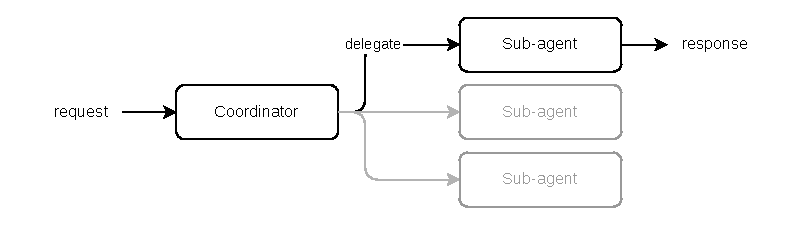
\includegraphics[width=0.9\textwidth]{images/routing_response_direct.pdf}
	\caption[Direct response]{Delegation. The selected sub-agent returns its response straight to the requester; the coordinator does not see it.}
	\label{fig:routing-direct}
\end{figure}

\begin{figure}[ht]
	\centering
	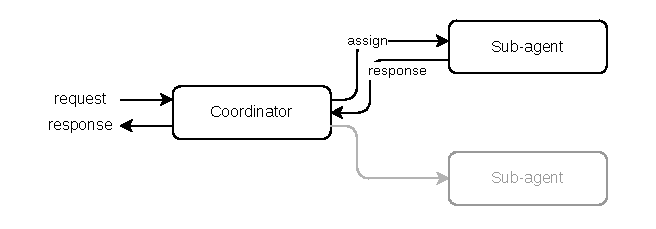
\includegraphics[width=0.74\textwidth]{images/routing_response_coordinator.pdf}
	\caption[Coordinator-mediated response]{Assignment. The selected sub-agent returns its response to the coordinator, which elaborates the final response sent to the requester.}
	\label{fig:routing-coordinator}
\end{figure}

\subsection{Separable and overlapping specialization}
\label{subsec:separable-overlapping}

What the routing decision has to resolve depends on how the sub-agents relate to each other. The sub-agents may cover disjoint subject matter, and in this case the wording of a request separates them. A support system with a billing agent and a shipping agent is of this kind: a request that mentions an invoice or a refund belongs to the billing agent, and a request that mentions a package or a delivery date belongs to the shipping agent. The two agents rarely share vocabulary, so the classification is straightforward from the text alone.

By contrast, in other systems the sub-agents may cover the same subject matter, or subject matters that are closely related. In this case, the wording of a request becomes harder to map to the right one. A travel-booking system with an agent dedicated to the lowest fare and a separate agent dedicated to the shortest travel time is of this kind: both agents can receive a request about the same flight, and the wording of the request might not, by itself, indicate which of the two constraints the requester meant to prioritize.

The same effect is documented in intent classification. ATIS and SNIPS are two datasets of task-oriented dialog utterances. Each utterance is labeled with its \emph{intent class}, the category of goal it expresses, such as \emph{flight} or \emph{airfare} \cite{bihaniFuzzyClassificationMultiintent2021}. Bihani and Rayz compared classification accuracy across the two and reported that it depends on the lexical overlap between the classes \cite{bihaniFuzzyClassificationMultiintent2021}. In ATIS, phrases such as \emph{show me} and \emph{from} repeat across different intent classes; accuracy on it is lower and more variable than on SNIPS, where utterances of different intents share fewer words \cite{bihaniFuzzyClassificationMultiintent2021}. They gave the utterances \emph{show me flights to Philadelphia coming from Baltimore}, labeled as the intent \emph{flight}, and \emph{show me airlines with flights from Denver}, labeled as the intent \emph{airline}, as an example of this overlap \cite{bihaniFuzzyClassificationMultiintent2021}. Higher lexical overlap between the classes lowers the accuracy with which an utterance is mapped to the correct one. This is the same difficulty that a coordinator faces when the sub-agents that it selects among cover overlapping subject matter, as in the fare and travel-time example above.

This extends to multi-turn scenarios. In conversational systems, a request is not necessarily self-contained: the element that fixes which sub-agent should handle it can appear in an earlier turn rather than in the last one. The context relevant to the routing decision is then spread across turns alternated between the user and the assistant, which adds the task of gathering that context to the difficulty of overlapping vocabulary described above.

\subsection{Downstream dependence on the routing decision}
\label{subsec:downstream-dependence}

The coordinator is the causally earliest step of the coordinator pattern described above, and the only one whose output determines which other component runs at all. Once the request has been handed to a sub-agent, no later step reopens the selection. An error made by the coordinator is therefore inherited by everything computed after it. The sub-agent applies its own criteria to a request that should have been handled under different criteria, and its output can be internally consistent while still addressing the wrong problem.

A wrong routing decision is therefore a problem of \emph{trajectory}: the correctness of a run is a property of the whole sequence of steps, and a wrong step early in it is not repaired by anything that follows. It is one instance of a broader problem in evaluating agents, discussed in Chapter~\ref{chap:evaluating-agents}.

